\documentclass{article} % For LaTeX2e
\usepackage{iclr2020_conference,times}

% Optional math commands from https://github.com/goodfeli/dlbook_notation.
%%%%% NEW MATH DEFINITIONS %%%%%

\usepackage{amsmath,amsfonts,bm}

% Mark sections of captions for referring to divisions of figures
\newcommand{\figleft}{{\em (Left)}}
\newcommand{\figcenter}{{\em (Center)}}
\newcommand{\figright}{{\em (Right)}}
\newcommand{\figtop}{{\em (Top)}}
\newcommand{\figbottom}{{\em (Bottom)}}
\newcommand{\captiona}{{\em (a)}}
\newcommand{\captionb}{{\em (b)}}
\newcommand{\captionc}{{\em (c)}}
\newcommand{\captiond}{{\em (d)}}

% Highlight a newly defined term
\newcommand{\newterm}[1]{{\bf #1}}


% Figure reference, lower-case.
\def\figref#1{figure~\ref{#1}}
% Figure reference, capital. For start of sentence
\def\Figref#1{Figure~\ref{#1}}
\def\twofigref#1#2{figures \ref{#1} and \ref{#2}}
\def\quadfigref#1#2#3#4{figures \ref{#1}, \ref{#2}, \ref{#3} and \ref{#4}}
% Section reference, lower-case.
\def\secref#1{section~\ref{#1}}
% Section reference, capital.
\def\Secref#1{Section~\ref{#1}}
% Reference to two sections.
\def\twosecrefs#1#2{sections \ref{#1} and \ref{#2}}
% Reference to three sections.
\def\secrefs#1#2#3{sections \ref{#1}, \ref{#2} and \ref{#3}}
% Reference to an equation, lower-case.
\def\eqref#1{equation~\ref{#1}}
% Reference to an equation, upper case
\def\Eqref#1{Equation~\ref{#1}}
% A raw reference to an equation---avoid using if possible
\def\plaineqref#1{\ref{#1}}
% Reference to a chapter, lower-case.
\def\chapref#1{chapter~\ref{#1}}
% Reference to an equation, upper case.
\def\Chapref#1{Chapter~\ref{#1}}
% Reference to a range of chapters
\def\rangechapref#1#2{chapters\ref{#1}--\ref{#2}}
% Reference to an algorithm, lower-case.
\def\algref#1{algorithm~\ref{#1}}
% Reference to an algorithm, upper case.
\def\Algref#1{Algorithm~\ref{#1}}
\def\twoalgref#1#2{algorithms \ref{#1} and \ref{#2}}
\def\Twoalgref#1#2{Algorithms \ref{#1} and \ref{#2}}
% Reference to a part, lower case
\def\partref#1{part~\ref{#1}}
% Reference to a part, upper case
\def\Partref#1{Part~\ref{#1}}
\def\twopartref#1#2{parts \ref{#1} and \ref{#2}}

\def\ceil#1{\lceil #1 \rceil}
\def\floor#1{\lfloor #1 \rfloor}
\def\1{\bm{1}}
\newcommand{\train}{\mathcal{D}}
\newcommand{\valid}{\mathcal{D_{\mathrm{valid}}}}
\newcommand{\test}{\mathcal{D_{\mathrm{test}}}}

\def\eps{{\epsilon}}


% Random variables
\def\reta{{\textnormal{$\eta$}}}
\def\ra{{\textnormal{a}}}
\def\rb{{\textnormal{b}}}
\def\rc{{\textnormal{c}}}
\def\rd{{\textnormal{d}}}
\def\re{{\textnormal{e}}}
\def\rf{{\textnormal{f}}}
\def\rg{{\textnormal{g}}}
\def\rh{{\textnormal{h}}}
\def\ri{{\textnormal{i}}}
\def\rj{{\textnormal{j}}}
\def\rk{{\textnormal{k}}}
\def\rl{{\textnormal{l}}}
% rm is already a command, just don't name any random variables m
\def\rn{{\textnormal{n}}}
\def\ro{{\textnormal{o}}}
\def\rp{{\textnormal{p}}}
\def\rq{{\textnormal{q}}}
\def\rr{{\textnormal{r}}}
\def\rs{{\textnormal{s}}}
\def\rt{{\textnormal{t}}}
\def\ru{{\textnormal{u}}}
\def\rv{{\textnormal{v}}}
\def\rw{{\textnormal{w}}}
\def\rx{{\textnormal{x}}}
\def\ry{{\textnormal{y}}}
\def\rz{{\textnormal{z}}}

% Random vectors
\def\rvepsilon{{\mathbf{\epsilon}}}
\def\rvtheta{{\mathbf{\theta}}}
\def\rva{{\mathbf{a}}}
\def\rvb{{\mathbf{b}}}
\def\rvc{{\mathbf{c}}}
\def\rvd{{\mathbf{d}}}
\def\rve{{\mathbf{e}}}
\def\rvf{{\mathbf{f}}}
\def\rvg{{\mathbf{g}}}
\def\rvh{{\mathbf{h}}}
\def\rvu{{\mathbf{i}}}
\def\rvj{{\mathbf{j}}}
\def\rvk{{\mathbf{k}}}
\def\rvl{{\mathbf{l}}}
\def\rvm{{\mathbf{m}}}
\def\rvn{{\mathbf{n}}}
\def\rvo{{\mathbf{o}}}
\def\rvp{{\mathbf{p}}}
\def\rvq{{\mathbf{q}}}
\def\rvr{{\mathbf{r}}}
\def\rvs{{\mathbf{s}}}
\def\rvt{{\mathbf{t}}}
\def\rvu{{\mathbf{u}}}
\def\rvv{{\mathbf{v}}}
\def\rvw{{\mathbf{w}}}
\def\rvx{{\mathbf{x}}}
\def\rvy{{\mathbf{y}}}
\def\rvz{{\mathbf{z}}}

% Elements of random vectors
\def\erva{{\textnormal{a}}}
\def\ervb{{\textnormal{b}}}
\def\ervc{{\textnormal{c}}}
\def\ervd{{\textnormal{d}}}
\def\erve{{\textnormal{e}}}
\def\ervf{{\textnormal{f}}}
\def\ervg{{\textnormal{g}}}
\def\ervh{{\textnormal{h}}}
\def\ervi{{\textnormal{i}}}
\def\ervj{{\textnormal{j}}}
\def\ervk{{\textnormal{k}}}
\def\ervl{{\textnormal{l}}}
\def\ervm{{\textnormal{m}}}
\def\ervn{{\textnormal{n}}}
\def\ervo{{\textnormal{o}}}
\def\ervp{{\textnormal{p}}}
\def\ervq{{\textnormal{q}}}
\def\ervr{{\textnormal{r}}}
\def\ervs{{\textnormal{s}}}
\def\ervt{{\textnormal{t}}}
\def\ervu{{\textnormal{u}}}
\def\ervv{{\textnormal{v}}}
\def\ervw{{\textnormal{w}}}
\def\ervx{{\textnormal{x}}}
\def\ervy{{\textnormal{y}}}
\def\ervz{{\textnormal{z}}}

% Random matrices
\def\rmA{{\mathbf{A}}}
\def\rmB{{\mathbf{B}}}
\def\rmC{{\mathbf{C}}}
\def\rmD{{\mathbf{D}}}
\def\rmE{{\mathbf{E}}}
\def\rmF{{\mathbf{F}}}
\def\rmG{{\mathbf{G}}}
\def\rmH{{\mathbf{H}}}
\def\rmI{{\mathbf{I}}}
\def\rmJ{{\mathbf{J}}}
\def\rmK{{\mathbf{K}}}
\def\rmL{{\mathbf{L}}}
\def\rmM{{\mathbf{M}}}
\def\rmN{{\mathbf{N}}}
\def\rmO{{\mathbf{O}}}
\def\rmP{{\mathbf{P}}}
\def\rmQ{{\mathbf{Q}}}
\def\rmR{{\mathbf{R}}}
\def\rmS{{\mathbf{S}}}
\def\rmT{{\mathbf{T}}}
\def\rmU{{\mathbf{U}}}
\def\rmV{{\mathbf{V}}}
\def\rmW{{\mathbf{W}}}
\def\rmX{{\mathbf{X}}}
\def\rmY{{\mathbf{Y}}}
\def\rmZ{{\mathbf{Z}}}

% Elements of random matrices
\def\ermA{{\textnormal{A}}}
\def\ermB{{\textnormal{B}}}
\def\ermC{{\textnormal{C}}}
\def\ermD{{\textnormal{D}}}
\def\ermE{{\textnormal{E}}}
\def\ermF{{\textnormal{F}}}
\def\ermG{{\textnormal{G}}}
\def\ermH{{\textnormal{H}}}
\def\ermI{{\textnormal{I}}}
\def\ermJ{{\textnormal{J}}}
\def\ermK{{\textnormal{K}}}
\def\ermL{{\textnormal{L}}}
\def\ermM{{\textnormal{M}}}
\def\ermN{{\textnormal{N}}}
\def\ermO{{\textnormal{O}}}
\def\ermP{{\textnormal{P}}}
\def\ermQ{{\textnormal{Q}}}
\def\ermR{{\textnormal{R}}}
\def\ermS{{\textnormal{S}}}
\def\ermT{{\textnormal{T}}}
\def\ermU{{\textnormal{U}}}
\def\ermV{{\textnormal{V}}}
\def\ermW{{\textnormal{W}}}
\def\ermX{{\textnormal{X}}}
\def\ermY{{\textnormal{Y}}}
\def\ermZ{{\textnormal{Z}}}

% Vectors
\def\vzero{{\bm{0}}}
\def\vone{{\bm{1}}}
\def\vmu{{\bm{\mu}}}
\def\vtheta{{\bm{\theta}}}
\def\va{{\bm{a}}}
\def\vb{{\bm{b}}}
\def\vc{{\bm{c}}}
\def\vd{{\bm{d}}}
\def\ve{{\bm{e}}}
\def\vf{{\bm{f}}}
\def\vg{{\bm{g}}}
\def\vh{{\bm{h}}}
\def\vi{{\bm{i}}}
\def\vj{{\bm{j}}}
\def\vk{{\bm{k}}}
\def\vl{{\bm{l}}}
\def\vm{{\bm{m}}}
\def\vn{{\bm{n}}}
\def\vo{{\bm{o}}}
\def\vp{{\bm{p}}}
\def\vq{{\bm{q}}}
\def\vr{{\bm{r}}}
\def\vs{{\bm{s}}}
\def\vt{{\bm{t}}}
\def\vu{{\bm{u}}}
\def\vv{{\bm{v}}}
\def\vw{{\bm{w}}}
\def\vx{{\bm{x}}}
\def\vy{{\bm{y}}}
\def\vz{{\bm{z}}}

% Elements of vectors
\def\evalpha{{\alpha}}
\def\evbeta{{\beta}}
\def\evepsilon{{\epsilon}}
\def\evlambda{{\lambda}}
\def\evomega{{\omega}}
\def\evmu{{\mu}}
\def\evpsi{{\psi}}
\def\evsigma{{\sigma}}
\def\evtheta{{\theta}}
\def\eva{{a}}
\def\evb{{b}}
\def\evc{{c}}
\def\evd{{d}}
\def\eve{{e}}
\def\evf{{f}}
\def\evg{{g}}
\def\evh{{h}}
\def\evi{{i}}
\def\evj{{j}}
\def\evk{{k}}
\def\evl{{l}}
\def\evm{{m}}
\def\evn{{n}}
\def\evo{{o}}
\def\evp{{p}}
\def\evq{{q}}
\def\evr{{r}}
\def\evs{{s}}
\def\evt{{t}}
\def\evu{{u}}
\def\evv{{v}}
\def\evw{{w}}
\def\evx{{x}}
\def\evy{{y}}
\def\evz{{z}}

% Matrix
\def\mA{{\bm{A}}}
\def\mB{{\bm{B}}}
\def\mC{{\bm{C}}}
\def\mD{{\bm{D}}}
\def\mE{{\bm{E}}}
\def\mF{{\bm{F}}}
\def\mG{{\bm{G}}}
\def\mH{{\bm{H}}}
\def\mI{{\bm{I}}}
\def\mJ{{\bm{J}}}
\def\mK{{\bm{K}}}
\def\mL{{\bm{L}}}
\def\mM{{\bm{M}}}
\def\mN{{\bm{N}}}
\def\mO{{\bm{O}}}
\def\mP{{\bm{P}}}
\def\mQ{{\bm{Q}}}
\def\mR{{\bm{R}}}
\def\mS{{\bm{S}}}
\def\mT{{\bm{T}}}
\def\mU{{\bm{U}}}
\def\mV{{\bm{V}}}
\def\mW{{\bm{W}}}
\def\mX{{\bm{X}}}
\def\mY{{\bm{Y}}}
\def\mZ{{\bm{Z}}}
\def\mBeta{{\bm{\beta}}}
\def\mPhi{{\bm{\Phi}}}
\def\mLambda{{\bm{\Lambda}}}
\def\mSigma{{\bm{\Sigma}}}

% Tensor
\DeclareMathAlphabet{\mathsfit}{\encodingdefault}{\sfdefault}{m}{sl}
\SetMathAlphabet{\mathsfit}{bold}{\encodingdefault}{\sfdefault}{bx}{n}
\newcommand{\tens}[1]{\bm{\mathsfit{#1}}}
\def\tA{{\tens{A}}}
\def\tB{{\tens{B}}}
\def\tC{{\tens{C}}}
\def\tD{{\tens{D}}}
\def\tE{{\tens{E}}}
\def\tF{{\tens{F}}}
\def\tG{{\tens{G}}}
\def\tH{{\tens{H}}}
\def\tI{{\tens{I}}}
\def\tJ{{\tens{J}}}
\def\tK{{\tens{K}}}
\def\tL{{\tens{L}}}
\def\tM{{\tens{M}}}
\def\tN{{\tens{N}}}
\def\tO{{\tens{O}}}
\def\tP{{\tens{P}}}
\def\tQ{{\tens{Q}}}
\def\tR{{\tens{R}}}
\def\tS{{\tens{S}}}
\def\tT{{\tens{T}}}
\def\tU{{\tens{U}}}
\def\tV{{\tens{V}}}
\def\tW{{\tens{W}}}
\def\tX{{\tens{X}}}
\def\tY{{\tens{Y}}}
\def\tZ{{\tens{Z}}}


% Graph
\def\gA{{\mathcal{A}}}
\def\gB{{\mathcal{B}}}
\def\gC{{\mathcal{C}}}
\def\gD{{\mathcal{D}}}
\def\gE{{\mathcal{E}}}
\def\gF{{\mathcal{F}}}
\def\gG{{\mathcal{G}}}
\def\gH{{\mathcal{H}}}
\def\gI{{\mathcal{I}}}
\def\gJ{{\mathcal{J}}}
\def\gK{{\mathcal{K}}}
\def\gL{{\mathcal{L}}}
\def\gM{{\mathcal{M}}}
\def\gN{{\mathcal{N}}}
\def\gO{{\mathcal{O}}}
\def\gP{{\mathcal{P}}}
\def\gQ{{\mathcal{Q}}}
\def\gR{{\mathcal{R}}}
\def\gS{{\mathcal{S}}}
\def\gT{{\mathcal{T}}}
\def\gU{{\mathcal{U}}}
\def\gV{{\mathcal{V}}}
\def\gW{{\mathcal{W}}}
\def\gX{{\mathcal{X}}}
\def\gY{{\mathcal{Y}}}
\def\gZ{{\mathcal{Z}}}

% Sets
\def\sA{{\mathbb{A}}}
\def\sB{{\mathbb{B}}}
\def\sC{{\mathbb{C}}}
\def\sD{{\mathbb{D}}}
% Don't use a set called E, because this would be the same as our symbol
% for expectation.
\def\sF{{\mathbb{F}}}
\def\sG{{\mathbb{G}}}
\def\sH{{\mathbb{H}}}
\def\sI{{\mathbb{I}}}
\def\sJ{{\mathbb{J}}}
\def\sK{{\mathbb{K}}}
\def\sL{{\mathbb{L}}}
\def\sM{{\mathbb{M}}}
\def\sN{{\mathbb{N}}}
\def\sO{{\mathbb{O}}}
\def\sP{{\mathbb{P}}}
\def\sQ{{\mathbb{Q}}}
\def\sR{{\mathbb{R}}}
\def\sS{{\mathbb{S}}}
\def\sT{{\mathbb{T}}}
\def\sU{{\mathbb{U}}}
\def\sV{{\mathbb{V}}}
\def\sW{{\mathbb{W}}}
\def\sX{{\mathbb{X}}}
\def\sY{{\mathbb{Y}}}
\def\sZ{{\mathbb{Z}}}

% Entries of a matrix
\def\emLambda{{\Lambda}}
\def\emA{{A}}
\def\emB{{B}}
\def\emC{{C}}
\def\emD{{D}}
\def\emE{{E}}
\def\emF{{F}}
\def\emG{{G}}
\def\emH{{H}}
\def\emI{{I}}
\def\emJ{{J}}
\def\emK{{K}}
\def\emL{{L}}
\def\emM{{M}}
\def\emN{{N}}
\def\emO{{O}}
\def\emP{{P}}
\def\emQ{{Q}}
\def\emR{{R}}
\def\emS{{S}}
\def\emT{{T}}
\def\emU{{U}}
\def\emV{{V}}
\def\emW{{W}}
\def\emX{{X}}
\def\emY{{Y}}
\def\emZ{{Z}}
\def\emSigma{{\Sigma}}

% entries of a tensor
% Same font as tensor, without \bm wrapper
\newcommand{\etens}[1]{\mathsfit{#1}}
\def\etLambda{{\etens{\Lambda}}}
\def\etA{{\etens{A}}}
\def\etB{{\etens{B}}}
\def\etC{{\etens{C}}}
\def\etD{{\etens{D}}}
\def\etE{{\etens{E}}}
\def\etF{{\etens{F}}}
\def\etG{{\etens{G}}}
\def\etH{{\etens{H}}}
\def\etI{{\etens{I}}}
\def\etJ{{\etens{J}}}
\def\etK{{\etens{K}}}
\def\etL{{\etens{L}}}
\def\etM{{\etens{M}}}
\def\etN{{\etens{N}}}
\def\etO{{\etens{O}}}
\def\etP{{\etens{P}}}
\def\etQ{{\etens{Q}}}
\def\etR{{\etens{R}}}
\def\etS{{\etens{S}}}
\def\etT{{\etens{T}}}
\def\etU{{\etens{U}}}
\def\etV{{\etens{V}}}
\def\etW{{\etens{W}}}
\def\etX{{\etens{X}}}
\def\etY{{\etens{Y}}}
\def\etZ{{\etens{Z}}}

% The true underlying data generating distribution
\newcommand{\pdata}{p_{\rm{data}}}
% The empirical distribution defined by the training set
\newcommand{\ptrain}{\hat{p}_{\rm{data}}}
\newcommand{\Ptrain}{\hat{P}_{\rm{data}}}
% The model distribution
\newcommand{\pmodel}{p_{\rm{model}}}
\newcommand{\Pmodel}{P_{\rm{model}}}
\newcommand{\ptildemodel}{\tilde{p}_{\rm{model}}}
% Stochastic autoencoder distributions
\newcommand{\pencode}{p_{\rm{encoder}}}
\newcommand{\pdecode}{p_{\rm{decoder}}}
\newcommand{\precons}{p_{\rm{reconstruct}}}

\newcommand{\laplace}{\mathrm{Laplace}} % Laplace distribution

\newcommand{\E}{\mathbb{E}}
\newcommand{\Ls}{\mathcal{L}}
\newcommand{\R}{\mathbb{R}}
\newcommand{\emp}{\tilde{p}}
\newcommand{\lr}{\alpha}
\newcommand{\reg}{\lambda}
\newcommand{\rect}{\mathrm{rectifier}}
\newcommand{\softmax}{\mathrm{softmax}}
\newcommand{\sigmoid}{\sigma}
\newcommand{\softplus}{\zeta}
\newcommand{\KL}{D_{\mathrm{KL}}}
\newcommand{\Var}{\mathrm{Var}}
\newcommand{\standarderror}{\mathrm{SE}}
\newcommand{\Cov}{\mathrm{Cov}}
% Wolfram Mathworld says $L^2$ is for function spaces and $\ell^2$ is for vectors
% But then they seem to use $L^2$ for vectors throughout the site, and so does
% wikipedia.
\newcommand{\normlzero}{L^0}
\newcommand{\normlone}{L^1}
\newcommand{\normltwo}{L^2}
\newcommand{\normlp}{L^p}
\newcommand{\normmax}{L^\infty}

\newcommand{\parents}{Pa} % See usage in notation.tex. Chosen to match Daphne's book.

\DeclareMathOperator*{\argmax}{arg\,max}
\DeclareMathOperator*{\argmin}{arg\,min}

\DeclareMathOperator{\sign}{sign}
\DeclareMathOperator{\Tr}{Tr}
\let\ab\allowbreak


\usepackage{hyperref}
\usepackage{url}

\usepackage{amsmath}
\usepackage{amssymb}
\usepackage{wasysym}
\usepackage{amsthm}
\usepackage{graphicx}

\newtheorem{theorem}{Theorem}[section]
\newtheorem{definition}{Definition}[section]
\newtheorem{lemma}[theorem]{Lemma}
\newtheorem{proposition}[theorem]{Proposition}
\newtheorem{corollary}[theorem]{Corollary}
\newtheorem{assumption}[definition]{Assumption}
\newtheorem{conjecture}[theorem]{Conjecture}
\newtheorem{remark}[theorem]{Remark}


\title{Global graph curvature}

% Authors must not appear in the submitted version. They should be hidden
% as long as the \iclrfinalcopy macro remains commented out below.
% Non-anonymous submissions will be rejected without review.

\author{Antiquus S.~Hippocampus, Natalia Cerebro \& Amelie P. Amygdale \thanks{ Use footnote for providing further information
about author (webpage, alternative address)---\emph{not} for acknowledging
funding agencies.  Funding acknowledgements go at the end of the paper.} \\
Department of Computer Science\\
Cranberry-Lemon University\\
Pittsburgh, PA 15213, USA \\
\texttt{\{hippo,brain,jen\}@cs.cranberry-lemon.edu} \\
\And
Ji Q. Ren \& Yevgeny LeNet \\
Department of Computational Neuroscience \\
University of the Witwatersrand \\
Joburg, South Africa \\
\texttt{\{robot,net\}@wits.ac.za} \\
\AND
Coauthor \\
Affiliation \\
Address \\
\texttt{email}
}

% The \author macro works with any number of authors. There are two commands
% used to separate the names and addresses of multiple authors: \And and \AND.
%
% Using \And between authors leaves it to \LaTeX{} to determine where to break
% the lines. Using \AND forces a linebreak at that point. So, if \LaTeX{}
% puts 3 of 4 authors names on the first line, and the last on the second
% line, try using \AND instead of \And before the third author name.

\newcommand{\fix}{\marginpar{FIX}}
\newcommand{\new}{\marginpar{NEW}}

%\iclrfinalcopy % Uncomment for camera-ready version, but NOT for submission.
\begin{document}


\maketitle

\begin{abstract}
Recently, non-Euclidean spaces became popular for embedding structured data. However, determining the suitable curvature for a given dataset is still an open problem. 
In this paper, we define a notion of global graph curvature and analyze a problem of estimating this curvature using only graph-based characteristics (without actual embedding). 
We review the existing notions of local curvature (e.g., Ollivier-Ricci curvature) and show that they are often unable to estimate the global one. 
Hence, we propose a new estimator of global graph curvature which increases the quality of graph embeddings.
\end{abstract}

\section{Introduction}

\textbf{[To be written later]}

\section{Background and related work}

\paragraph{Embeddings} 
\textbf{[Basic information about what is embedding. Some selected relevant papers on embeddings and their applications.]}

\paragraph{Fidelity measures} \textbf{[Define distortion and MAP. Discuss minuses of distortion (practical and theoretical). Define threshold-based loss.]}

\paragraph{Hyperbolic and Spherical Spaces} \textbf{[Discuss hyperbolic and spherical spaces and their main properties which we will use throughout the proofs.]}

\paragraph{Embeddings into non-eucledian spaces} \textbf{[Discuss representative examples for embeddings into various spaces.]}

\section{Local graph curvatures}

There are several different notions of local graph curvature proposed in the literature. Many of them are based on the notion of sectional curvature and Ricci curvature defined for Riemannian manifolds. Intuitively, Ricci curvature controls whether the distance between small spheres is smaller or larger than the distance between the centers of the spheres. 
Ricci curvature is positive if
small spheres are closer than their centers are.
%Ricci curvature can also be understood as representing the amount by which the volume of a geodesic ball in a curved Riemannian manifold deviates from that of the standard ball in Euclidean space. 
%If Ricci curvature at a point is non-negative, the volume growth with respect to the radius of the ball centered at this point is a polynomial; if the Ricci curvature is negative everywhere, the volume growth is exponential. 
\textbf{[Probably rewrite and give a reference to the formal definition of Ricci curvature]}

\subsection{Ollivier curvature}

Ollivier's coarse Ricci curvature translates the definition of Ricci curvature to graphs. 
Again, the idea is to compare the distances between two small balls with the
distance between their centers. 
The distance between balls is defined by the well-known optimal transport
distance (a.k.a. Wasserstein distance, earth-mover distance,
Monge-Kantorovich-Rubinstein distance).

Formally, for a graph $G$ we consider the shortest path metric on $G$, denoted by $d_G$, and let $W_1^G$ denote the Wasserstein metric with respect to the metric space $(G,d_G)$. Furthermore, for each node $v$ let $m_v$ denote the uniform probability measure on the neighbors of $v$, i.e., $m_v(u) = \frac{1_{u \sim v}}{\mathrm{deg}(v)}$, where $\mathrm{deg}(v)$ denotes the degree of $v$. Then, the classic definition of Ollivier curvature between two neighboring nodes $v \sim u$ in $G$ is defined as
\begin{equation}\label{eq:def_classic_ollivier_graphs}
	\kappa_G(u,v) = 1 - W_1^G(m_v, m_u).
\end{equation}

It is important to note that Ollivier curvature is defined in much more generality in terms of metrics and random walks, see~\citep{ollivier2009ricci}. Thus, different version on graphs can be considered. \Eqref{eq:def_classic_ollivier_graphs} corresponds to the classical choices of graph distance and random walk on the graph.

%\textbf{[Should we discuss the convergence of Ollivier curvature to the curvature of the underlying manifold? Let us discuss whether it can strengthen the paper or not (probably not).]}
%The strength of Ollivier-Ricci curvature lies in the fact that when we consider its continuous version on Riemannian manifolds than this converges to the Ricci curvature, see~\cite[Example 7]{ollivier2009ricci}. It turns out that this also holds when we consider dense random geometric graphs on Riemannian manifolds (upcoming paper). However, for this one needs to deviate from the classical version and consider random-walks on larger neighborhoods. Still these results highlights that Ollivier-Ricci curvature can properly encode the curvature of the underlying manifold. 



\subsection{Forman curvature}

Another notion of graph curvature called Forman curvature~\citep{sreejith2016forman} is based on the discretization of Ricci curvature proposed by~\citet{forman2003bochner}. It is defined for general weighted graph $G$, with both vertex weights $w(v)$ and edge weights $w(u,v)$, as follows
\begin{equation}\label{eq:forman}
	F_G(u,v) = w(u,v) \left(\frac{w(u) + w(v)}{w(u,v)} - \hspace{-8pt}\sum_{u^\prime \in N(u)\setminus v}  \frac{w(u)}{w(u,u^\prime)} - \hspace{-8pt} \sum_{v^\prime \in N(v) \setminus u} \frac{w(v)}{w(v,v^\prime)}\right),
\end{equation}
where $N(v)$ denotes the neighborhood of a node $v$. 
When the graph $G$ is not weighted, i.e., when $w(v) = 1 = w(v,u)$ for all nodes $v$ and edges $(u,v)$, we get
\begin{equation}\label{eq:forman2}
F_G(u,v) = \left(2 - (\mathrm{deg}(v) - 1) - (\mathrm{deg}(u) - 1)\right) = 4 - (\mathrm{deg}(v) + \mathrm{deg}(u)).
\end{equation}

The general formula by Forman included the faces of any dimension, which can be done for graphs as well~\citep{weber2017coarse}. In~\Eqref{eq:forman} only $1$-dimensional faces (edges) are included. However, one can also include $2$-dimensional faces. This was considered in~\cite{samal2018comparative}, where $2$-dimensional faces on three nodes (triangles) were considered. In the case of an unweighted graph we then obtain
\begin{equation}\label{eq:def_forman_curvature_triangles}
	\hat F_G(u,v) = F(u,v) + 3\Delta_{uv} 
	= 4 - \mathrm{deg}(v) - \mathrm{deg}(u) + 3\Delta_{uv},
\end{equation}
where $\Delta_{uv}$ is the number of triangles that contain the edge $(u,v)$. 

\subsection{Approximate Ollivier curvature}

\textbf{[Say something on complexity of computing Ollivier curvature? I think that we should discuss this approximation only if it gives a significant boost in speed.]}

An explicit formula for Ollivier-Ricci curvature in graphs is obtained by~\citet{kelly2019self} under somewhat restrictive assumptions. 
For an edge $(u,v)$, let $\triangle_{uv}$, $\square_{uv}$ and $\pentagon_{uv}$ denote, respectively, the number of triangles, squares and pentagons in the graph that include the edge $(u,v)$. Moreover let $a \wedge b = \min\{a,b\}$, $a \vee b = \max\{a,b\}$ and $[a]^+ = a \vee 0$. Then we define:
\begin{multline}\label{eq:def_ollivier_ricci_approx}
		\kappa_G^\ast(u,v) = \frac{\triangle_{uv}}{\mathrm{deg}(u) \wedge \mathrm{deg}(v)} 
			- \left[1 - \frac{1 + \triangle_{uv} + \square_{uv}}{\mathrm{deg}(u) \vee \mathrm{deg}(v)} - \frac{1}{\mathrm{deg}(u) \wedge \mathrm{deg}(v)}\right]^+\\
	- \left(\frac{\triangle_{uv}}{\mathrm{deg}(u) \vee \mathrm{deg}(v)} 
			- \frac{\triangle_{uv}}{\mathrm{deg}(u) \wedge \mathrm{deg}(v)}\right) \vee \left(1 - \frac{1 + \triangle_{uv} + \square_{uv} + \pentagon_{uv}}
			{\mathrm{deg}(u) \vee \mathrm{deg}(v)}
			- \frac{1}{\mathrm{deg}(u) \wedge \mathrm{deg}(v)}\right).
\end{multline}

\citet{kelly2019self} shows that $\kappa_G^\ast(u,v) = \kappa_G(u,v)$ if and only if short cycles of length $3$, $4$ or $5$ that include the edge $(u,v)$ share no other edges. For example, if $w$ is a neighbor of both $u$ and $v$ (so $w$ is part of a $3$-cycle) then $w$ cannot be connected to any other neighbor of either $u$ or $v$, since that would mean that $w$ is part of a $4$-cycle that includes the edge $(u,v)$. Although this requirement is quite restrictive, one could still use~\Eqref{eq:def_ollivier_ricci_approx} as an approximation (or even a definition) of local curvature in graphs.

\subsection{Heuristic sectional curvature}

A different notion of curvature used by \citep{gu2019learning} is based on the following geometric fact. 
Let $abc$ be a geodesic triangle and let $m$ be the (geodesic) midpoint of $bc$, then the value
\begin{equation}\label{eq:parallelogram_law}
	d(a,m)^2 + \frac{d(b,c)^2}{4} - \frac{d(a,b)^2 + d(a,c)^2}{2}
\end{equation}
is equal to zero in euclidean space, is positive in spherical space and negative in hyperbolic space.

For graphs, let $v$ be a node in $G$, $b,c$ neighbors of $v$ and $a$ any other node. Then we define
\begin{equation}
\xi_G(v;b,c;a) = \frac{1}{2 d(a,v)} \left( 	d(a,v)^2 + \frac{d(b,c)^2}{4} - \frac{d(a,b)^2 + d(a,c)^2}{2} \right).
\end{equation}
This resembles~\Eqref{eq:parallelogram_law} with $m = v$. Additionally, the normalization constant $2d_G(v,a)$ is included to yield the right scalings for trees and cycles.
To define the graph sectional curvature of a node $v$ and its neighbors $b,c$ we average $\xi_G(v;b,c;a)$ over all possible $a$: 
$\xi_G(v; b,c) = \frac{1}{|G|-3} \sum_{a \in G\setminus \{v,b,c\}} \xi_G(v;b,c;a)$.\footnote{[Add comment about the fact that we do not let $a$ conincide with $b$ or $c$.]}

%The curvature of the graph is then defined as the average of $\xi_G(v; u,w)$. This is computed as $\xi_G = \frac{\xi_G(v^\ast,u^\ast,w^\ast,z^\ast)}{2d_G(v^\ast,z^\ast)}$, where $v^\ast, u^\ast, w^\ast$ and $z^\ast$ are selected uniformly at random from $G$, $N(v^\ast)$, $N(v^\ast)\setminus u^\ast$ and $G\setminus v^\ast$, respectively. Here $N(v)$ denotes the neighborhood of $v$.

\section{Global graph curvature}

\textbf{[Some notation are inconsistent, will be improved]}

\subsection{Definition}

While there are many different notions of \textit{local} graph curvature, they cannot be easily used in practical application. In practice, data is usually embedded in a space of constant curvature, so a \textit{global} notion of curvature is needed. 
In this paper, we propose a practice-driven definition of global graph curvature and compute this curvature in some simple cases.

For a graph $G$ let $f(G)$ be the embedding of this graph into some metric space. Assume that we are given a loss function $L(f(G),G)$ for embedding task. For example, $L$ can be distortion or threshold-based loss. 
Now, let $L_{opt}(G,d,c)$ be the optimal loss for embedding in a space of dimension $d$ and curvature $c$:
\[
L_{opt}(G,d,c) = \min_{f(G)} L(f(G),G).
\]
Then, we can define a $d$-dimensional curvature of $G$ in the following way:
\[
C_{d}^{L}(G) = \argmin_C L_{opt}(G,d,c)\,.
\]
Note that there may be several values of curvature $c$ delivering a minimum of $L_{opt}(G,d,c)$, in this case we say that  $C_{d}^{L}(G)$ consists of all such points.

\textbf{[At some point we should mention that we ignore precision problem. The only way I can see how we can take precision into account is to choose the maximum value among the set $C_d^L(G)$.]}

\subsection{Approximations}

\textbf{[Discuss that all local curvatures can potentially be used to define global one, just by averaging.]} 

\textbf{[Also, define our new curvature.]}

\textbf{[Add a table with complexities.]}

\subsection{Theoretical analysis of global curvature and its approximations}

\subsubsection{Star on $n+1$ nodes}

It is known that trees are negatively curved. 
We analyze this theoretically for two loss functions. We start the simplest tree of depth 1 on $n+1$ nodes (one parent node and $n$ leaves).

\paragraph{Ollivier curvature} 
Consider any tree graph $T$, let $v \sim u$ be two neighbors. Then Proposition 2 in~\citep{jost2014ollivier} states that
\begin{equation}\label{eq:ollivier_tree}
	\kappa_T(u,v) = -2\left(1 - \frac{1}{\mathrm{deg}(v)} - \frac{1}{\mathrm{deg}(u)}\right)^+, 
\end{equation}
where $t^+ = \max\{0,t\}$. In particular, if either $\mathrm{deg}(v) = 1$ or $\mathrm{deg}(u) = 1$, then $\kappa_T(u,v) = 0$.  As a result, for a star-graph $G$, we have $\kappa_G(u,v) = 0$ for all edges, so the average value is $\kappa_G = 0$.

\paragraph{Forman curvature}
If follows from \Eqref{eq:forman} and \Eqref{eq:forman2} that
$F_G = \hat F_G = 3-n$ (Forman curvature is the same for all edges).

\paragraph{Approximate Ollivier curvature} According to \Eqref{eq:def_ollivier_ricci_approx}, $\kappa_G^* = 0$.

\paragraph{Heuristic sectional curvature}

Sectional curvature is defined for a node and its two neighbors, in case of a star we can only take a central node $v$ and two neighboring one $u$ and $w$. In this case, for any other node $z$, we obtain $\xi_G(v;u,w;z) = -1$. Therefore, by averaging we obtain $\xi_G = -1$.

\paragraph{Distortion-based curvature} 
We prove the following theorem (the proof is in Appendix).

\begin{theorem}\label{thm:star_distortion}
In hyperbolic space, for any $d$, we have $D(G) = \Omega\left(\frac{1}{n\sqrt{-c}}\right)$ and there exists such embedding that $D(G) = O\left(\frac{\log n}{\sqrt{-c}}\right)$. Therefore, for any given graph $G$, we have $C_{G,d} = -\infty$.
\end{theorem}

\textbf{[Comment that we do not consider euclidean and spherical spaces, but they do not affect the main conclusion.]}

\textbf{[Describe the basic intuition about why trees are hard to embed in any space if we care about distortion.]}

\paragraph{Threshold-based curvature} 
For this curvature, the following theorem holds (proof is in Appendix).

\begin{theorem}\label{thm:star_threshold}
$C_d(G) = (-\infty, C)$.
\end{theorem}

\textbf{[I have analytic expression for $C$ if $d = 2$ (see Appendix). For $d > 2$ we have to use some results on sphere coding / kissing number.]}

\subsubsection{Infinite tree with branching factor $b$}

For symmentry, assume that the first node has $b+1$ children, while all other nodes have a parent and $b$ children.

\paragraph{Ollivier curvature} We can use \Eqref{eq:ollivier_tree} and get, for any edge,
$\kappa_G(u,v) = -2 \left(1 - \frac{1}{b+1} - \frac{1}{b+1} \right) = - 2 + \frac{4}{b+1}$. So, $\kappa_G = -2 + \frac{4}{b+1}$.

\paragraph{Forman curvature} 
It is easy to see that we have 
$F_G = \hat F_G = 4 - 2(b+1) = 2(1-b)$


\paragraph{Approximate Ollivier curvature} 
$\kappa_G^\ast(u,v) = -2 + \frac{4}{b+1}$.

\paragraph{Heuristic sectional curvature} For each sectional curvature, we average 0 and 1. \textbf{[Can try to compute precisely for a finite tree or reference to their paper.]}

\paragraph{Distortion-based curvature} 

\begin{theorem}\label{thm:tree_distortion} $C_{G,d} = -\infty$.
\end{theorem}

\textbf{[The fact that the tree is infinite makes this statement harder, I have to think about it.]}

\paragraph{Threshold-based curvature} 

\begin{theorem}\label{thm:tree_threshold}
$C_d(G) = (-\infty, C)$.
\textbf{[we also need some bounds on $C$]}
\end{theorem}



\subsubsection{Cycle of size $n$} 

\paragraph{Ollivier curvature}  
$\kappa_G(u,v) = 0$ for all edges, so by averaging we obtain $0$.

\paragraph{Forman curvature} 

$F(u,v) = 0 = F_2(u,v)$.

\paragraph{Approximate Ollivier curvature} 

$\kappa_G^* = 0$.

\paragraph{Heuristic sectional curvature} \textbf{[ToDo]}

\paragraph{Distortion-based curvature} For any dimension $d$ and for $n \ge 4$, there is a unique curvature which gives zero distortion:
\[
C_d(G) = \left(\frac{2\pi}{n}\right)^2.
\]
This is easy to explain: if we consider three consequent vertices, then the middle one should lie on the geodetic between the other two. So, they all lie on a great circle (of length $n$).

\paragraph{Threshold-based curvature} 
Here, again, we have $C_d(G) = (-\infty, C)$ with some $C>0$. It is easy to prove that any curvature $c < \left(\frac{4\pi}{n}\right)^2$ is ok, but I have to think whether we can get some larger bound. 

\subsubsection{Complete graph on $n$ vertices}

\paragraph{Ollivier curvature}  
$\kappa_G(u,v) = \frac{n-2}{n-1}$, so average is the same.

\paragraph{Forman curvature} 

$F(u,v) = 6 - 2n$, $F_2(u,v) = n$.

\paragraph{Approximate Ollivier curvature} 

$\kappa_G^* = 0$.

\paragraph{Heuristic sectional curvature} 

$\kappa_G^* = ...$. \textbf{[Easy, but did not do yet. We can see the difference with Ollivier with this example.]}

\paragraph{Distortion-based curvature}

Assume that $d = n-2$, then it is easy to find $C_d(G)$. Note that we want to get $n-1$-simplex, which can be embedded into a $n-2$-dimensional spherical space, the radius is $R = a\sqrt{\frac{n-1}{2n}}$, and we want
\[
2 R \arcsin \frac{a}{2R} = 1.
\]
\[
2 a\sqrt{\frac{n-1}{2n}} \arcsin \sqrt{\frac{n}{2(n-1)}} = 1.
\]
\[
a  = \sqrt{\frac{2n}{(n-1)}}\frac{1}{2\arcsin \sqrt{\frac{n}{2(n-1)}}}.
\]
\[
R = \frac{1}{2\arcsin \sqrt{\frac{n}{2(n-1)}}}
\]

so we have
\[
C_{n-2}(G) = 4 \left(\arcsin \sqrt{\frac{n}{2(n-1)}}\right)^2\,.
\]

Also, it seems that for all $n$ and $d$ curvature $-\infty$ gives zero distortion since we can make a star from a clique using one Steiner node.

\paragraph{Threshold-based curvature} We can embed cliques to any space (all nodes to one point).

\subsubsection{Complete bipartite graph $K_{l,m}$}

W.l.o.g. we assume that $l \ge m \ge 2$ (the remaining cases are stars and are already considered).

\paragraph{Ollivier curvature}  
\textcolor{red}{[Pim, do you know if there are any results about Ollivier curvature of bipartite graphs?]}

\paragraph{Forman curvature} 

$F(G) = \hat F(G) = 4 - l - m$. Again, Forman curvature can be highly negative.

\paragraph{Approximate Ollivier curvature} 
In is easy to derive from \Eqref{eq:def_ollivier_ricci_approx} that $\kappa^*(G) = 0$. \textcolor{red}{[Which is porbably significantly different from true Ollivier curvature.]}

\paragraph{Heuristic sectional curvature} If $v$ and $a$ are in the same part of the bipartite graph, then $\xi_G(v;b,c;a) = 1$, otherwise $\xi_G(v;b,c;a) = -1$. Therefore, if $a$ belongs to the part of size $l$, sectional curvature is
$\xi_G(v;b,c) = \frac{l-m+1}{l+m-3}$, otherwise it is $\xi_G(v;b,c) = \frac{m-l+1}{l+m-3}$. As a result, by averaging over all triplets, we get
\[
\xi(G) = \frac{1}{l \binom{m}{2} + m \binom{l}{2}} \left(l \binom{m}{2} \frac{l-m+1}{l+m-3} + m \binom{l}{2} \frac{m-l+1}{l+m-3}\right) = \frac{2ml - m^2 - l^2 + m + l - 2}{(m+l-2)(l+m-3)}.
\]
In particular, if $m = l$ we get $\xi(G) = \frac{1}{2m - 3}$. In other words, for balanced complete bipartite graphs $\xi(G)$ is positive, but tends to zero as graph grows.

\paragraph{Distortion-based curvature} 

Figure~\ref{fig:bipartite} shows empirical behavior of distortion depending on curvature. We observe that for all graphs optimal curvature is between 2 and 2.5. 
The following proposition gives an intuition about why one could expect this. 

\begin{proposition}\label{prop:bipartite_distortion}
For any $d$, $C_d^{dist}(K_{2,2}) = \left(\frac{\pi}{2}\right)^2 \approx 2.47$ and $K_{2,2}$ is the only complete bipartite graph (with at least two nodes in each part) for which zero distortion is achievable.
\end{proposition}

Indeed, the result for $K_{2,2}$ follows from Proposition~\ref{prop:cycle_distortion}. Moreover, if for $K_{l,m}$ we have $l \ge 3$ and $m \ge 2$, then ...
 
\section{Experiments}

\begin{figure}
    \centering
    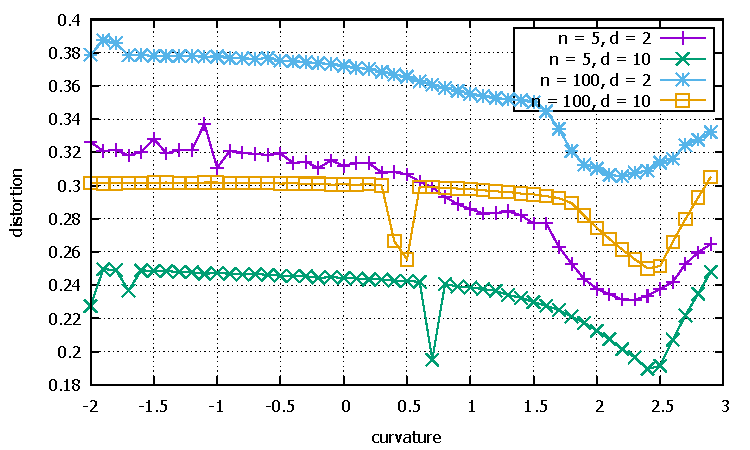
\includegraphics[width = 0.49 \textwidth]{bipartite_distortion.pdf}
    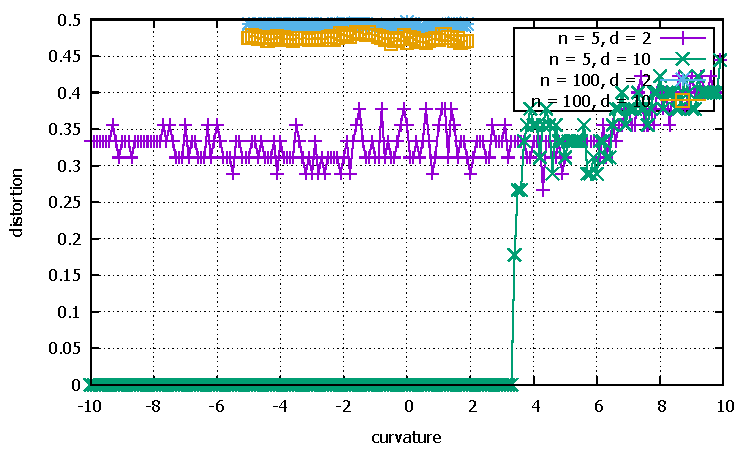
\includegraphics[width = 0.49 \textwidth]{bipartite_zero_one.pdf}
    \caption{Complete bipartite graphs $K_{n,n}$}
    \label{fig:bipartite}
\end{figure}

\textbf{[Below I describe the current status of experiments. I will start writing a better version of this part on weekends.]}

\subsection{Experiments on synthetic graphs}

For synthetic graphs, in most cases, we know what to expect and where is the optimal curvature. So, these experiments are expected to illustrate our theoretical observations. 

In all experiments, we consider two dimensions: $d = 2$ and $d = 10$.

\begin{itemize}
    \item Star on $n+1$ nodes, $n = 5$ and $n = 10$. Loss: distortion. 
    We want to illustrate the claim $C = -\infty$, i.e., to show that loss function decreases when $C$ becomes smaller. This experiment is done. 
    \item Star on $n+1$ nodes, $n = 5$ and $n = 10$. Loss: zero-one. Here we want to show that optimal curvature is at most some constant. Which is about 1.23 for $n=5$, $d = 2$ and $-1.2$ for $n = 7$, $d = 2$ (we add this pair to illustrate negative curvature). This experiment is noisy (small graphs + discrete metric), but done. 
    \item Cycle on $n+1$ nodes, $n = 5$, $n = 100$. Loss: distortion. We want to illustrate that global curvature do not depend on distortion. For $n = 5$ we have about 1.6, for $n = 100$ we have $n = 0.004$. This experiment is done.
    \item Cycle on $n+1$ nodes, $n = 5$, $n = 100$. Loss: zero-one. Want to show that can be embedded in any curvature smaller than some positive value (we need enough space). This experiment is done.
    \item Clique on $n$ nodes, $n = 5$, $n = 100$. Loss: distortion. We also add here $n = 4$ for $d = 2$ and $n = 12$ for $d = 10$. In two latter cases, We want to illustrate the following theoretical result: optimum is in some positive curvature (we have a formula, which agrees with figure) and in $-\infty$ (we see that error decreases for smaller curvatures). This experiment is done.
   \item Clique on $n$ nodes, $n = 5$, $n = 100$. Loss: zero-one. Trivial experiment (zero loss), finished, will not add to the paper.
   \item Tree with branching factor $3$ and depth $6$. Loss: distortion. Very nice plot, optimal distortion is about $-1/4$ for both $d$. This contradicts my initial intuition. \textbf{[TODO: explain the optimal curvature!]}
   \item Tree with branching factor $3$ and depth $6$. Loss: zero-one. Slightly strange result: for $d = 0$ good curvature is 0 and below  (I expected more negative one). 
   \item Complete bipartite graph, $n/2 = 5$, $n/2 = 100$. Loss: distortion. Interesting result, positive curvature (2-2.5), don't have theory for that. Plus some unexpected drop at about 0.5 on two plots... This experiment is done for now. 
   \item Complete bipartite graph, $n/2 = 5$, $n/2 = 100$. Loss: zero-one. \textbf{[Will be finished after I have some bound for curvature]} 
\end{itemize}

\subsection{Experiments on real graphs}

For now, we just run experiments on datasets of reasonable size and see how the plots look like. 

\begin{itemize}
    \item Karate, $n = 32$ \textbf{[almost done, on embeddings]}
    \item Conflict \textbf{[Done for zero-one, problem for distortion, discuss and fix?]}
    \item CSPhDs \textbf{[Done for distortion, in progress for zero-one, on embeddings]}
    
\end{itemize}


\section{Conclusion}

\textbf{[To be added after the main parts are completed.]}

%\begin{table}[t]
%\caption{Sample table title}
%\label{sample-table}
%\begin{center}
%\begin{tabular}{ll}
%\multicolumn{1}{c}{\bf PART}  %&\multicolumn{1}{c}{\bf DESCRIPTION}
%\\ \hline \\
%Dendrite         &Input terminal \\
%Axon             &Output terminal \\
%Soma             &Cell body (contains cell nucleus) \\
%\end{tabular}
%\end{center}
%\end{table}

%\subsubsection*{Author Contributions}

%\subsubsection*{Acknowledgments}

\bibliography{references}
\bibliographystyle{iclr2020_conference}

\appendix

\section{Distortion-based curvature for simple graphs}

\subsection{Proof of Theorem~\ref{thm:star_distortion} (star on $n+1$ node)}

The idea of the proof is the following: we take any curvature $C$ and prove a lower bound on distortion (for given dimension $d$). Then, we obtain an upper bound on distortion which tends to zero as $C \to -\infty$, which gives the claimed result.

Let us analyze the lower bound for distortion. Recall that distortion of a graph is average distortion over all pairs of nodes. Let $v$ be the central node and $v_1, \ldots, v_n$ be its neighbors. Then,
\begin{multline*}
D(G) = \frac{1}{\binom{n+1}{2}} \left( \sum_{v_i} {|d(f(v),f(v_i)) - 1|} + \sum_{v_i \neq v_j} \frac{|d(f(v_i),f(v_j)) - 2|}{2} \right) \\
= \frac{1}{\binom{n+1}{2}} \sum_{1 \le i_1 < i_2 < i_3 \le n} \left(
\sum_{1\le j \le 3}  \frac{|d(f(v_{i_j}),f(v)) - 1|}{{n-1 \choose 2}} +
\sum_{1\le j < k\le 3}  \frac{|d(f(v_{i_j}),f(v_{i_k})) - 2|}{2(n-2)}   \right).
\end{multline*}

Let $D_{min}$ be the lower bound for the following weighted distortion for the star with 3 leaves:
\[
D_{min} = \min_{f} \sum_{1\le j \le 3}  \frac{|d(f(v_j),f(v)) - 1|}{(n-1)/4} +
\sum_{1\le j < k\le 3}  |d(f(v_j),f(v_k)) - 2|,
\]
then 
\[
D(G) \ge \frac{{n\choose 3}}{2(n-2){n+1 \choose 2}} D_{min} = \frac{ (n-1)D_{min}}{6(n+1)}\,.
\]
Hence, it remains to find a lower bound on $D_{min}$, i.e., a lower bound for a weighted distortion for a star with central node $v$ and three leaves $v_1, v_2, v_3$.
If we consider three angles at the node $v$, then at least one of them is $\alpha \le 2 \pi / 3$, so we can get a lower bound only for this triangle, which is, w.l.o.g., formed by $v, v_1, v_2$.  Namely,
\[
D_{min} \ge  |d(f(v_1),f(v_2)) - 2| + \frac{|d(f(v_1),f(v)) - 1| + |d(f(v_2),f(v)) - 1|}{(n-1)/2} .
\]


Further we give a detailed proof for hyperbolic space, but it is easy to show that in spherical and euclidean spaces $D_{min}$ is even larger.

Denote $d(f(v_1),f(v)) = x = 1 + \varepsilon$, $d(f(v_2),f(v)) = y = 1 + \delta$, $d(f(v_1),f(v)) = z = 2 + \varepsilon + \delta - \varphi$ with some $\varepsilon, \delta$ and some $\varphi > 0$ (from triangle inequality). Assume that $|\varepsilon| < 1/2$ and $|\delta| < 1/2$ (otherwise the lower bound is trivial). We can use the hyperbolic law of cosines (denote $R = \frac{1}{\sqrt{-c}}$):
\[
\cosh \frac{z}{R} = \cosh \frac{x}{R} \cosh \frac{y}{R} - \sinh \frac{x}{R} \sinh \frac{y}{R} \cos \alpha,
\]
from which we get 
\[
\cosh \frac{x+y}{R} - \cosh \frac{z}{R} = \sinh \frac{x}{R} \sinh \frac{y}{R} (1 - \cos \alpha) = \Omega\left(e^{(x+y)/R}\right).
\]
It follows from the above equation that 
$e^{\frac{x+y-z}{R}} - 1 = \Omega\left(e^{\frac{x+y-z}{R}}\right) = \Omega(1)$, so $\varphi = x + y - z = \Omega(R)$.

Note that $D_{min} \ge |z-2| + \frac{|x-1| + |y-1|}{(n-1)/2} =  |\varepsilon + \delta - \varphi| + \frac{|\varepsilon| + |\delta|}{(n-1)/2}$. This gives us a lower bound $D_{min} = \Omega(R/n) = \Omega\left(\frac{1}{n\sqrt{-c}}\right)$, so $D(G) =  \Omega\left(\frac{1}{n\sqrt{-c}}\right)$.

Let us analyze upper bound for distortion. To do this, we want to find some embedding with sufficiently low distortion. 

%\textbf{[I had two ideas how to prove the upper bound. The first one is to distribute leaves uniformly on a 2-dimensional circle, the second~--- to sample them uniformly on a $d$-dimensional hyper-sphere and then compute the expected distortion. For now I choose the first approach since it is easier.]}

Let $v$ be the central node, then we spread all other nodes uniformly on a 2-dimensional circle of radius $1$ centred at $v$. The smallest angle between two points is $2 \pi / n$. Therefore, the distance between leaves is at least $d$ with
\[
\cosh \frac{d}{R} = 1  + \left(1 -  \cos \frac{2 \pi}{n}\right)  \sinh^2 \frac{1}{R} \,.
\]


So, our loss (distortion) can be lower bounded by
\begin{multline*}
D(G) \le \frac{{n \choose 2}}{2{n+1\choose 2}} \left(2 - R\cdot \mathrm{arccosh}\left( \left(1 - \cos \frac{2 \pi}{n}\right)\sinh^2\frac{1}{R}  + 1 \right)\right) \\
= \frac{(n-1)}{2(n+1)} \left(2 - R\cdot \mathrm{arccosh}\left( \left(1 - \cos \frac{2 \pi}{n}\right)\sinh^2\frac{1}{R}  + 1 \right)\right)
\end{multline*}
Note that $1 - \cos\frac{2\pi}{n} = \Theta\left(\frac{1}{n}\right)$ and $\sinh^2\left(\frac{1}{R}\right) = \Theta\left(e^{2/R}\right)$.
Then, $\textrm{arccosh}\left(\Theta\left(\frac{1}{n} e^{2/R}\right) + 1 \right)$ behaves as $\sqrt{2e^{2/R}/n}$ if $2/R \ll \log n$ and as $\frac{2}{R} - \log n$ if $2/R \gg \log n$.
Therefore, we get
\[
D(G) = O\left( R \log n \right) = O\left( \frac{\log n}{\sqrt{-c}} \right).
\]

\section{Threshold-based curvature for simple graphs}

\subsection{Proof of Theorem~\ref{thm:star_threshold} (star on $n+1$ node)}

We want to find an embedding which gives zero error (or correlation 1). This means that all leaves have to be inside the ball of radius 1 around the central node $v$ and also the distance between any two leaves has to be larger than one. 

It is easy to see that if we managed to spread $n$ points inside the ball of radius 1 with distances more than 1 between them, then we can move each point along the radius up to distance 1 from $v$ preserving this property. Therefore, it is sufficient to spread all points on a hypersphere. 

Let us first consider $d = 2$. In this case we can find an explicit analytic expression for $C$.

Assume that $n > 6$. It is clear that in this case we have to consider only hyperbolic space, since $n$ neighbors would not fit to a circle of radius 1 in neither spherical or euclidean space.

$C$ is just the largest curvature which allows to have distance exactly 1 between closest leaves. Let us find $C$. We use hyperbolic low of cosines again and let $C = -\frac{1}{R^2}$, $\alpha = \frac{2\pi}{n}$:
%\[
%\cosh{\frac{1}{k}} = \cosh^2{\frac{1}{k}} - \sinh^2{\frac{1}{k}}\cos\alpha.
%\]
%\[
%\cosh{\frac{1}{k}} = 1 +  (1- \cos\alpha) \sinh^2{\frac{1}{k}}.
%\]
%\[
%\cosh{\frac{1}{k}} = 1 +  2\sin^2 \frac{\alpha}{2} \sinh^2{\frac{1}{k}}.
%\]
%\[
%\frac{1}{2\sin^2 \frac{\alpha}{2}} = \frac{\sinh^2{\frac{1}{k}}}{\cosh{\frac{1}{k}} - 1}.
%\]
%\[
%\frac{1}{2\sin \frac{\alpha}{2}} = \frac{\sinh{\frac{1}{k}}}{\sqrt{2}\sqrt{\cosh{\frac{1}{k}} - 1}}.
%\]
\[
\cosh\frac{1}{2R} = \frac{1}{2\sin \frac{\alpha}{2}},
\]
\[
R = \frac{1}{2\,\textrm{arccosh}\frac{1}{2\sin \frac{\alpha}{2}}},
\]
\[
C = - \left(2\,\textrm{arccosh}\frac{1}{2\sin \frac{\alpha}{2}}\right)^2.
\]
Obviously, for any $c < C$ we can spread $n$ neighbors in a required way.

Note that if $n$ is large, then $\sin \frac{\alpha}{2} = \sin\frac{\pi}{n-1} \sim \frac{\pi}{n-1}$. Then,  $\textrm{arccosh}\frac{1}{2\sin \frac{\alpha}{2}} \sim \textrm{arccosh}\frac{n-1}{2\pi} \sim \log n$, so we get $C \sim - 4 \log^2 n$. 

Now, let us consider $n \le 6$. Obviously, for $n = 6$ we have $C = 0$.

If $n < 6$, then $C > 0$. Let $C = \frac{1}{R^2}$, $\alpha = \frac{2\pi}{n}$. Similarly to the hyperbolic case, we now have:
\[
\cos{\frac{1}{R}} = \frac{\cos \alpha}{1 - \cos \alpha},
\]
\[
C = \left(\arccos \frac{\cos \alpha}{1 - \cos \alpha}\right)^2.
\]

Now, let us consider $d > 2$. In this case, we only have lower and upper bounds on $C$. 

\textbf{Use spherical code / kissing number} 

%About upper bound. If we have $n$ points at distance at least 1 from each other, then the spheres of radius 1/2 around them do no intersect. Therefore, we can find the volume that we need to get such spheres. 

%For $d > 2$ we can get lower and upper bounds for $C$. One bound we can obtain by covering the surface of a unit ball by the balls of radius $1/2$. The other bound can be obtained by using spherical packing. \textbf{[To be finished formally.]} 

\subsection{Proof of Theorem~\ref{thm:tree_threshold} (tree with branching factor $b$)}

First, let us discuss the upper bound. 
Here we say that all children at levels $l, l-2, l-4, \ldots$ have to fit to the ball of radius $l$ with all pairwise distances $> 1$. We can consider large enough $l$ here (and get hyperbolic space).

\begin{figure}
    \centering
    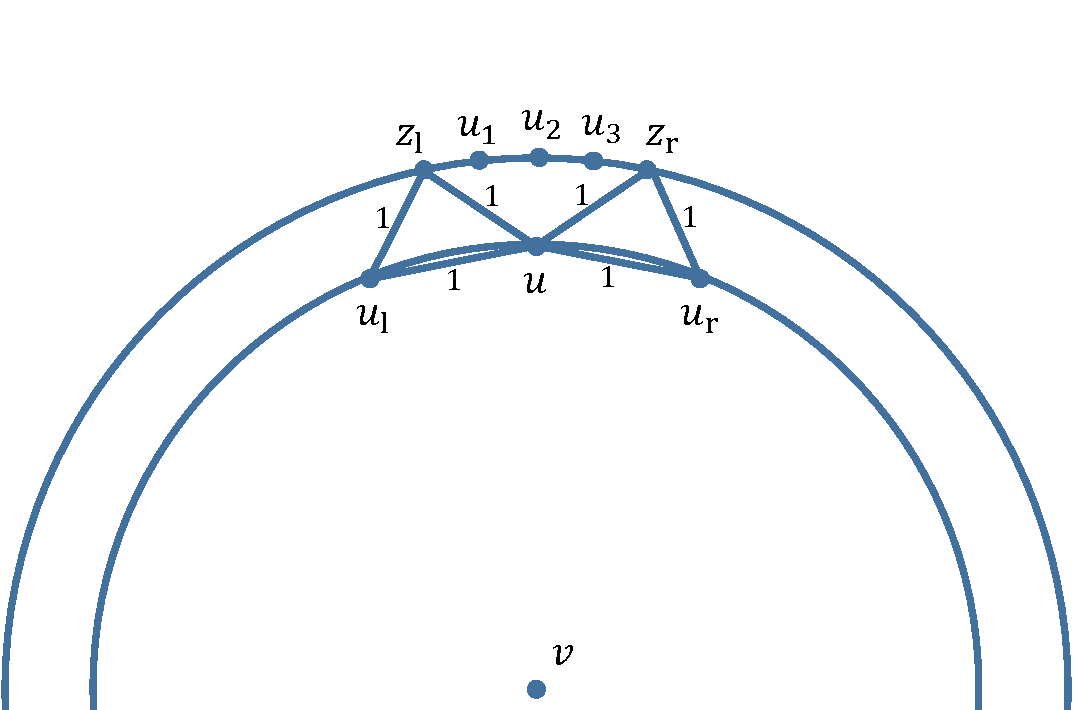
\includegraphics[width = 0.5 \textwidth]{trees.pdf}
    \caption{Threshold-based embedding of trees}
    \label{fig:trees}
\end{figure}


For the lower bound, we have to guarantee that embedding exists. For this, we provide the following construction (see Figure~\ref{fig:trees} for an illustration).
(Below we assume that the curvature is large enough for our construction to work, then we estimate the required curvature.)
First, we take the node $v$ and consider a circle of radius 1 around this node. 
We spread $b + 1$ neighbors uniformly around this node. For our construction to work, we need all distances between these nodes to be larger than 1.
Now, at some step of the algorithm, assume that we have all nodes at level $l$ to be placed at some circle centered at $v$, all distances between the nodes at level $l$ are larger than 1, our aim is to find positions for all nodes level $l + 1$. 

Let us take any node at $l$-th level. Consider two points $u_l$ and $u_r$ on the same circle at distance 1 from the node $u$ to the left and to the right, respectively.
Let $u,u_l,z_l$ and $u,u_r,z_r$ for equilateral triangles (with sides equal to 1). Then we let the points at $l+1$-th level to be spread on the circle centred at $v$ and passing through $z_l$ and $z_r$. The children of $u$ ($u_1, \ldots, u_{b}$) will be placed on the circular arc between $z_l$ and $z_r$. As usual, we want $u_i$ and $u_{i+1}$ to be at distance at least 1 from each other. Moreover, they have to be at distance at least 1 from children of other nodes. Also, note that placing $u_1, \ldots, u_{b}$ between $z_l$ and $z_r$ guarantees that these nodes are closer than 1 to their parent node $u$ but at the same time at a distance larger than 1 from all other nodes at $l$-th level. Also, all points at $l$-th level are far enough from points at $l+2$-th level.

It remains to find such maximum curvature that the required conditions are satisfied. Let $r$ and $r'$ be radii of circles at $l$-th and $l+1$-th levels and let $2\alpha = \angle u_l v u$. We know (the law of cosines and $\cos 2\alpha = 1 - 2\sin^2 \alpha$) that
\begin{equation}\label{eq:1}
\cosh \frac{1}{R} = 1 + 2 \sinh \frac{r}{R} \sin^2 \alpha \,.
\end{equation}
And the only condition we need for the whole procedure to work is that we have enough space on the circular arc for placing $b$ nodes there:
\[
\cosh \frac{1}{R} \le 1 + 2 \sinh \frac{r'}{R} \sin^2 \frac{\alpha}{b} \,.
\]
Now we note that $\sin^2 \frac{\alpha}{b} \ge \frac{\sin^2 \alpha}{b^2}$ for all $b \ge 1$. Therefore, it is sufficient to have
\begin{equation}\label{eq:2}
\cosh \frac{1}{R} \le 1 + 2 \sinh \frac{r'}{R} \cdot \frac{\sin^2 \alpha}{b^2} \,.
\end{equation}
Combining \Eqref{eq:1} and \Eqref{eq:1}, we obtain:
\[
\sinh \frac{r'}{R} \ge b^2 \cdot \sinh \frac{r}{R}.
\]
To achieve this, it is sufficient to have:
\[
\frac{r' - r}{R} \ge \log b,
\]
\[
R \le \frac{r' - r}{\log b}.
\]
It remains to find the lower bound for $r' - r$ and it is easy to see that $r' - r$ decreases with $r$. Therefore, it is sufficient to consider only the second step of the construction procedure, when we move from the circle of radius 1 to the next one. In this case, $r = 1$ and 
\[
r' = 2 \, \mathrm{arccosh} \frac{\cosh 1}{\cosh 1/2}.
\]
So, we have 
\[
-C = \frac{1}{R^2} \le \left( \frac{\log b}{2 \, \mathrm{arccosh} \frac{\cosh 1}{\cosh 1/2} - 1} \right)^2.
\]


\section{Distortion of Random Geometric Graphs}

\textbf{[Will see how the result will be reformulated if we rescale the graph to thresold one. Based on the obtained result, we will include this section or not.]}

Consider the random graph $G_n^r$ constructed by choosing $n$ points uniformly in the square $[\sqrt{n}/2, \sqrt{n}/2]$ and connecting two points $u$ and $v$ if $d(u,v) \le r$. For the remainder of this section we will assume that $r \ge 244 \sqrt{\log(n)}$, which is slightly larger than the threshold value $r_c = \sqrt{\log(n)/\pi}$ at which point the graph $G_n^r$ becomes connected a.a.s. and furthermore that $r \le \sqrt{n}/2$. We will identify nodes $v \in V$ with points and let $(x_v,y_v)$ denote their corresponding coordinates.

Clearly, the structure of the graph $G_n^r$ is completely determined by the coordinates $\{(x_v,y_v)\}_{v \in V}$ of the chosen points. Hence, the most natural and optimal embedding for this graph should be in the $2$-dimensional Euclidean plane using these original coordinates. However, if we do this then the distortion actually diverges.

We use the following result from~\citep{diaz2016relation} concerning the stretch in $G_n^r$:

\begin{theorem}\label{thm:stretch_rgg}
Let $G_n^r$ be constructed as above. Then, for each pair of nodes $u,v \in V$ with $d(u, v) > r$, there exists sequences $a_n^-, a_n^+ \to 0$, depending on $r$, such that the following holds with probability $1 - o(n^{-5/2})$:
\begin{enumerate}
\item If $d(u,v) \ge \max\{12\log(n)^{3/2}/r, 21 r \log(n)\}$:
\[
	d_G(u,v) \ge \left\lfloor \frac{d(u,v)}{r}\left(1 + a_n^-\right)\right\rfloor
\]
\item if $r \ge 224 \sqrt{\log(n)}$:
\[
	d_G(u,v) \le \left\lceil \frac{d(u,v)}{r}\left(1 + a_n^+\right)\right\rceil
\]
\end{enumerate}
\end{theorem}

\begin{lemma}
Let $f : V \to \mathbb{R}^2$ denote the embedding for the graph $G_n^r$ that assigns to each node $v$ it original coordinates $(x_v,y_v)$ and let $D_n(r)$ denote the distortion associated with this embedding. Then
\[
	\mathbb{E}[D_n(r)] = \Omega\left(\sqrt{\log(n)}\right).
\]
\end{lemma}

\begin{proof}
Let $S_n$ denote the event for which the statements of Theorem~\ref{thm:stretch_rgg} holds for all pairs $(u,v)$. Then since the probability that it holds for one pair is $1 - o(n^{-5/2})$, it follows that $\mathbb{P}(S_n) = 1 - o(n^{-1/2})$.

On the event $S_n$, it follows from the second statement of Theorem~\ref{thm:stretch_rgg} that for all $u,v$ with $d(u,v) > r$
\[
	\left|\frac{d(u,v)}{d_G(u,v)} - 1\right| \ge \frac{d(u,v)}{d_G(u,v)} - 1
	\ge \frac{r(d_G(u,v) - 1)}{d_G(u,v)(1+a_n^+)} - 1.
\]
Therefore, on the event $S_n$, we have that
\begin{align*}
	D_n(r) &= \frac{1}{\binom{n}{2}} \sum_{u \ne v} \left|\frac{d(u,v)}{d_G(u,v)} - 1\right|\\
	&\ge \frac{1}{\binom{n}{2}} \sum_{u \ne v \atop d(u,v) > r} \left|\frac{d(u,v)}{d_G(u,v)} - 1\right|\\
	&\ge \frac{1}{\binom{n}{2}} \sum_{u \ne v \atop d(u,v) > r} \left(\frac{r(d_G(u,v) - 1)}{d_G(u,v)(1+a_n^+)} - 1\right)\\
	&\ge \left(\frac{r}{1 + a_n^+} - \frac{r}{d_G(u,v)(1+a_n^+)}\right) 
		\frac{|\{u \ne v \, :\, d(u,v) > r\}|}{\binom{n}{2}} - 1\\
	&\ge \left(\frac{r}{1 + a_n^+} - \frac{r}{n(1+a_n^+)}\right) 
			\frac{|\{u \ne v \, :\, d(u,v) > r\}|}{\binom{n}{2}} - 1\\
	&\ge 224 \sqrt{\log(n)} \frac{1 - \frac{1}{n}}{1 + a_n^+} \frac{|\{u \ne v \, :\, d(u,v) > r\}|}{\binom{n}{2}} - 1.
\end{align*}
Next we note that since $224 \pi \log(n) \le \pi r^2 \le \pi n/4$, we have that the expected number of nodes at least a distance $r$ away from a given node is at least $(n - \pi r^2) = \Omega(n)$ (center) and at most $n - \pi r^2/4 = O(n)$ (the corners). We conclude that
\[
	\mathbb{E}[|\{u \ne v \, :\, d(u,v) > r\}|] = \Theta\left(\binom{n}{2}\right).
\]

The result now follows since
\begin{align*}
	\mathbb{E}[D_n(r)] &\ge \mathbb{E}[D_n(r) 1_{S_n}] \\
	&\ge 224 \sqrt{\log(n)} \frac{1 - \frac{1}{n}}{1 + a_n^+} 
		\frac{\mathbb{E}[|\{u \ne v \, :\, d(u,v) > r\}|]}{\binom{n}{2}}
		= \Omega(\sqrt{\log(n)}).
\end{align*}
\end{proof}


\end{document}





\section{Default Notation}

In an attempt to encourage standardized notation, we have included the
notation file from the textbook, \textit{Deep Learning}
\cite{goodfellow2016deep} available at
\url{https://github.com/goodfeli/dlbook_notation/}.  Use of this style
is not required and can be disabled by commenting out
\texttt{math\_commands.tex}.


\centerline{\bf Numbers and Arrays}
\bgroup
\def\arraystretch{1.5}
\begin{tabular}{p{1in}p{3.25in}}
$\displaystyle a$ & A scalar (integer or real)\\
$\displaystyle \va$ & A vector\\
$\displaystyle \mA$ & A matrix\\
$\displaystyle \tA$ & A tensor\\
$\displaystyle \mI_n$ & Identity matrix with $n$ rows and $n$ columns\\
$\displaystyle \mI$ & Identity matrix with dimensionality implied by context\\
$\displaystyle \ve^{(i)}$ & Standard basis vector $[0,\dots,0,1,0,\dots,0]$ with a 1 at position $i$\\
$\displaystyle \text{diag}(\va)$ & A square, diagonal matrix with diagonal entries given by $\va$\\
$\displaystyle \ra$ & A scalar random variable\\
$\displaystyle \rva$ & A vector-valued random variable\\
$\displaystyle \rmA$ & A matrix-valued random variable\\
\end{tabular}
\egroup
\vspace{0.25cm}

\centerline{\bf Sets and Graphs}
\bgroup
\def\arraystretch{1.5}

\begin{tabular}{p{1.25in}p{3.25in}}
$\displaystyle \sA$ & A set\\
$\displaystyle \R$ & The set of real numbers \\
$\displaystyle \{0, 1\}$ & The set containing 0 and 1 \\
$\displaystyle \{0, 1, \dots, n \}$ & The set of all integers between $0$ and $n$\\
$\displaystyle [a, b]$ & The real interval including $a$ and $b$\\
$\displaystyle (a, b]$ & The real interval excluding $a$ but including $b$\\
$\displaystyle \sA \backslash \sB$ & Set subtraction, i.e., the set containing the elements of $\sA$ that are not in $\sB$\\
$\displaystyle \gG$ & A graph\\
$\displaystyle \parents_\gG(\ervx_i)$ & The parents of $\ervx_i$ in $\gG$
\end{tabular}
\vspace{0.25cm}


\centerline{\bf Indexing}
\bgroup
\def\arraystretch{1.5}

\begin{tabular}{p{1.25in}p{3.25in}}
$\displaystyle \eva_i$ & Element $i$ of vector $\va$, with indexing starting at 1 \\
$\displaystyle \eva_{-i}$ & All elements of vector $\va$ except for element $i$ \\
$\displaystyle \emA_{i,j}$ & Element $i, j$ of matrix $\mA$ \\
$\displaystyle \mA_{i, :}$ & Row $i$ of matrix $\mA$ \\
$\displaystyle \mA_{:, i}$ & Column $i$ of matrix $\mA$ \\
$\displaystyle \etA_{i, j, k}$ & Element $(i, j, k)$ of a 3-D tensor $\tA$\\
$\displaystyle \tA_{:, :, i}$ & 2-D slice of a 3-D tensor\\
$\displaystyle \erva_i$ & Element $i$ of the random vector $\rva$ \\
\end{tabular}
\egroup
\vspace{0.25cm}


\centerline{\bf Calculus}
\bgroup
\def\arraystretch{1.5}
\begin{tabular}{p{1.25in}p{3.25in}}
% NOTE: the [2ex] on the next line adds extra height to that row of the table.
% Without that command, the fraction on the first line is too tall and collides
% with the fraction on the second line.
$\displaystyle\frac{d y} {d x}$ & Derivative of $y$ with respect to $x$\\ [2ex]
$\displaystyle \frac{\partial y} {\partial x} $ & Partial derivative of $y$ with respect to $x$ \\
$\displaystyle \nabla_\vx y $ & Gradient of $y$ with respect to $\vx$ \\
$\displaystyle \nabla_\mX y $ & Matrix derivatives of $y$ with respect to $\mX$ \\
$\displaystyle \nabla_\tX y $ & Tensor containing derivatives of $y$ with respect to $\tX$ \\
$\displaystyle \frac{\partial f}{\partial \vx} $ & Jacobian matrix $\mJ \in \R^{m\times n}$ of $f: \R^n \rightarrow \R^m$\\
$\displaystyle \nabla_\vx^2 f(\vx)\text{ or }\mH( f)(\vx)$ & The Hessian matrix of $f$ at input point $\vx$\\
$\displaystyle \int f(\vx) d\vx $ & Definite integral over the entire domain of $\vx$ \\
$\displaystyle \int_\sS f(\vx) d\vx$ & Definite integral with respect to $\vx$ over the set $\sS$ \\
\end{tabular}
\egroup
\vspace{0.25cm}

\centerline{\bf Probability and Information Theory}
\bgroup
\def\arraystretch{1.5}
\begin{tabular}{p{1.25in}p{3.25in}}
$\displaystyle P(\ra)$ & A probability distribution over a discrete variable\\
$\displaystyle p(\ra)$ & A probability distribution over a continuous variable, or over
a variable whose type has not been specified\\
$\displaystyle \ra \sim P$ & Random variable $\ra$ has distribution $P$\\% so thing on left of \sim should always be a random variable, with name beginning with \r
$\displaystyle  \E_{\rx\sim P} [ f(x) ]\text{ or } \E f(x)$ & Expectation of $f(x)$ with respect to $P(\rx)$ \\
$\displaystyle \Var(f(x)) $ &  Variance of $f(x)$ under $P(\rx)$ \\
$\displaystyle \Cov(f(x),g(x)) $ & Covariance of $f(x)$ and $g(x)$ under $P(\rx)$\\
$\displaystyle H(\rx) $ & Shannon entropy of the random variable $\rx$\\
$\displaystyle \KL ( P \Vert Q ) $ & Kullback-Leibler divergence of P and Q \\
$\displaystyle \mathcal{N} ( \vx ; \vmu , \mSigma)$ & Gaussian distribution %
over $\vx$ with mean $\vmu$ and covariance $\mSigma$ \\
\end{tabular}
\egroup
\vspace{0.25cm}

\centerline{\bf Functions}
\bgroup
\def\arraystretch{1.5}
\begin{tabular}{p{1.25in}p{3.25in}}
$\displaystyle f: \sA \rightarrow \sB$ & The function $f$ with domain $\sA$ and range $\sB$\\
$\displaystyle f \circ g $ & Composition of the functions $f$ and $g$ \\
  $\displaystyle f(\vx ; \vtheta) $ & A function of $\vx$ parametrized by $\vtheta$.
  (Sometimes we write $f(\vx)$ and omit the argument $\vtheta$ to lighten notation) \\
$\displaystyle \log x$ & Natural logarithm of $x$ \\
$\displaystyle \sigma(x)$ & Logistic sigmoid, $\displaystyle \frac{1} {1 + \exp(-x)}$ \\
$\displaystyle \zeta(x)$ & Softplus, $\log(1 + \exp(x))$ \\
$\displaystyle || \vx ||_p $ & $\normlp$ norm of $\vx$ \\
$\displaystyle || \vx || $ & $\normltwo$ norm of $\vx$ \\
$\displaystyle x^+$ & Positive part of $x$, i.e., $\max(0,x)$\\
$\displaystyle \1_\mathrm{condition}$ & is 1 if the condition is true, 0 otherwise\\
\end{tabular}
\egroup
\vspace{0.25cm}


\paragraph{Circle}

Consider a circle on $n$ nodes and let $v \sim u$ be two neighbors. Then $W_1^G(m_u,m_v) = 1$ and hence $\kappa_G(u,v) = 0$.



\paragraph{Lattice}
Consider the $2$-dimensional lattice $\mathbb{Z}^2$ and let $v \sim u$ be two neighbors. Then the optimal transportation from $m_u$ to $m_v$ is given by a translation by the vector $y - x$ and hence $W_1^G(m_v,m_u) = d_G(u,v) = 1$, see also \cite[Example 5]{ollivier2009ricci}, and thus $\kappa_G(u,v) = 0$.

\paragraph{Complete graph}

Consider a complete graph on $n$ nodes. Then, for any two nodes $u$ and $v$ it follows from Example 1 in~\cite{jost2014ollivier} that $\kappa_G(m_v, m_u) = \frac{n-2}{n-1} \to 1$ as $n \to \infty$.

\paragraph{Erd\H{o}s-Renyi graph}

The following results from~\cite{lin2011ricci} characterize Ollivier-Ricci curvature in $G(n,p)$:

\begin{enumerate}
\item If $p \ge \log(n)^{1/3} n^{-1/3}$ then almost surely
\[
	\kappa_G(u,v) = p + O\left(\sqrt{\frac{\log(n)}{n p}}\right).
\]
\item If $2 \log(n)^{1/2} n^{-1/2} \le p < \log(n)^{1/3} n^{-1/3}$ then almost surely
\[
	\kappa_G(u,v) = O\left(\frac{\log(n)}{n p^2}\right).
\]
\item If $\log(n)^{1/2} n^{-2/3} \ll p \ll \log(n)^{-1/2}$ then almost surely
\[
	\kappa_G(u,v) = -1 + O\left(n p^2\right) + O\left(\frac{\log(n)}{n^2 p^3}\right).
\]
\item If $\log(n) n^{-1} \ll p \ll n^{-2/3}$ then almost surely
\[
	\kappa_G(u,v) = -2 + O\left(n^2 p^3\right) + O\left(\sqrt{\frac{\log(n)}{np}}\right)
\]
\end{enumerate}